\documentclass[a4paper,10pt]{article}

% ---------------- PACCHETTI ----------------
\usepackage[utf8]{inputenc}       % encoding
\usepackage[T1]{fontenc}          % font encoding
\usepackage[italian]{babel}       % lingua italiana
\usepackage{graphicx}             % immagini
\usepackage{amsmath, amssymb}     % matematica
\usepackage{listings}             % codice sorgente
\usepackage{xcolor}               % colori
\usepackage{hyperref}             % link cliccabili
\usepackage{geometry}             % margini pagina
\usepackage{mdframed}
\usepackage{booktabs}
\usepackage{subcaption}
\usepackage{hyperref}
\usepackage{wrapfig}
\geometry{margin=2.5cm}

\newmdenv[linecolor=black,linewidth=0.5pt,backgroundcolor=white!10,
innertopmargin=10pt,
innerbottommargin=10pt,
innerleftmargin=10pt,
innerrightmargin=10pt]{citabox}
\definecolor{colorImportant}{HTML}{963428}

% ---------------- DOCUMENTO ----------------
\begin{document}
	
	\begin{titlepage}
		\centering
		\vspace*{\fill}
		\begin{figure}[h!]
			\centering
			\includegraphics[scale=3]{Resources/logo.pdf}
		\end{figure}
		\vspace{1cm}
		
		{\huge \textbf{Rifugio per adozione animali}}\\[0.5cm]
		{\Huge \textbf{\url{http://localhost/tmoretti/}}}\\[1.5cm]
		
		\rule{\textwidth}{0.5pt}\\[0.5cm] % linea orizzontale elegante
		{\LARGE Relazione di progetto}\\[0.1cm]
		\rule{\textwidth}{0.5pt}\\[2cm]
		
		\begin{flushright}
			{\Large \textbf{Università degli Studi di Padova}} \\[0.1cm]
			{\Large \textbf{L.T. in Informatica}} \\[0.1cm]
			{\Large \textbf{A.A. 2025/26}} \\[0.5cm]
		\end{flushright}
		
		\begin{flushleft}
			\textbf{2111001 (Referente)} Thomas Morettin (\href{mailto:thomas.morettin@studenti.unipd.it}{thomas.morettin@studenti.unipd.it}) \\
			\textbf{2111935} Felician Mario Necsulescu (\href{mailto:felicianmario.necsulescu@studenti.unipd.it}{felicianmario.necsulescu@studenti.unipd.it}) \\
			\textbf{2111947} Niccolò Feltrin (\href{mailto:niccolo.feltrin@studenti.unipd.it}{niccolo.feltrin@studenti.unipd.it}) \\ [0.5cm]
			\textbf{Data} 03.02.2026 \\
			\textbf{Corso} Tecnologie Web \\
			\textbf{\hspace*{0.5cm}Cod.} SCP4065581 \\
		\end{flushleft}
		\vspace{2cm}
		
		{\Large \textbf{Credenziali di accesso al sito}}
		\begin{table}[h!]
			\centering
			\begin{tabular}{lcc}
				\toprule
				\textbf{Ruolo} & \textbf{Username} & \textbf{Password} \\
				\midrule
				Amministratore & admin & admin
			\end{tabular}
		\end{table}
		\vspace*{\fill}
	\end{titlepage}
	\tableofcontents
	\clearpage
	
	\section{Scopo del sito}

	\textbf{Amici per Sempre} è una piattaforma web progettata per il rifugio di animali domestici situato a Padova. Il sito rappresenta la vetrina digitale della struttura e offre servizi completi sia per chi cerca un animale da adottare sia per chi ha necessità di affidare il proprio animale al rifugio.
    L'obiettivo principale è duplice:
	\begin{itemize}
		\item \textbf{Lato utenti}: permettere la consultazione degli animali ospitati, prenotare visite conoscitive per l'adozione e richiedere l'inserimento del proprio animale nel rifugio;
		\item \textbf{Lato rifugio}: gestire in modo efficiente le richieste di adozione, il calendario degli appuntamenti per visite e per l'accoglienza di nuovi animali.
	\end{itemize}
    Il portale si propone di creare un ponte bidirezionale: da un lato gli animali in cerca di famiglia incontrano i potenziali adottanti, dall'altro le persone che per vari motivi non possono più tenere il proprio animale trovano una soluzione responsabile attraverso l'affidamento al rifugio.
	\section{Analisi dei requisiti}
	\subsection{Analisi del target}
    Il sito è progettato per un'utenza eterogenea che include:
    \begin{itemize}
	\item \textbf{Potenziali adottanti}: persone di tutte le età in cerca di un animale da compagnia;
	\item \textbf{Proprietari in difficoltà}: cittadini che per motivi personali, economici o di salute necessitano di affidare il proprio animale a una struttura qualificata;
	\item \textbf{Visitatori curiosi}: utenti che desiderano conoscere la realtà del rifugio;
	\item \textbf{Amministratori}: personale del rifugio che gestisce richieste e appuntamenti.
    \end{itemize}
    Per garantire accessibilità universale, l'interfaccia adotta un linguaggio semplice, una gerarchia visiva chiara e una navigazione intuitiva, riducendo il carico cognitivo anche per utenti con competenze informatiche limitate o in situazioni di stress emotivo (come chi deve separarsi dal proprio animale).

    \subsection{Tipi di utente}
    Il sistema prevede due categorie principali di utenti con permessi differenziati:
    
    \vspace{1em}
    \textbf{Utente non autenticato:}
    \begin{itemize}
	   \item Visualizzazione degli animali disponibili per l'adozione con sistema di filtri avanzato;
	   \item Accesso alle informazioni sul rifugio e sulla missione;
	   \item Compilazione del form ``Porta in Adozione'' per richiedere un appuntamento e cedere il proprio animale;
	   \item Possibilità di consultare le schede dettagliate di ogni animale e prenotare una visita compilando un form.
    \end{itemize}

    \textbf{Utente autenticato (amministratore):}
    \begin{itemize}
	   \item Accesso all'area amministrativa con dashboard riepilogativa;
	   \item Gestione completa del calendario appuntamenti (visite per adozione + accoglienza animali esterni);
	   \item Visualizzazione e gestione dei ticket di richiesta adozione;
	   \item Gestione delle richieste di inserimento animali esterni nel rifugio;
    \end{itemize}

    \subsection{Funzionalità}
    Il portale offre un insieme articolato di funzionalità pensate per rispondere ai bisogni dei diversi tipi di utenti:

    \begin{itemize}
    \item \textbf{Catalogo animali dinamico.}  
    La sezione principale del sito consente la visualizzazione degli animali disponibili per l’adozione tramite un catalogo dinamico. Gli utenti possono filtrare i risultati per specie, sesso, età, taglia e carattere, oppure cercare un animale per nome tramite una barra di ricerca testuale. Un contatore aggiorna in tempo reale il numero di risultati visualizzati.

    \item \textbf{Schede dettagliate degli animali.}  
    Ogni animale dispone di una scheda dedicata contenente informazioni strutturate, una breve storia descrittiva e un elenco di caratteristiche comportamentali. I dati principali includono specie, età formattata automaticamente, sesso, peso, colore e razza, con particolare attenzione all’accessibilità tramite l’uso dell’attributo \texttt{lang} per razze con denominazione in lingua straniera.

    \item \textbf{Form ``Porta in Adozione''.}  
    Il sistema permette ai proprietari di animali di richiedere l’inserimento nel rifugio tramite un form guidato in tre fasi. Vengono raccolti i dati del proprietario e le informazioni principali sull’animale, con validazione sia lato client che lato server. Al termine della procedura viene inviata un’email di conferma e creato un appuntamento per la visita di accoglienza.

    \item \textbf{Sistema di prenotazione visite.}  
    Gli utenti autenticati possono prenotare una visita conoscitiva direttamente dalla scheda di un animale. Il form raccoglie i dati di contatto dell’utente e associa automaticamente la richiesta all’animale selezionato. A seguito dell’invio, il sistema genera un ticket di adozione e invia una conferma via email.

    \item \textbf{Dashboard amministrativa.}  
    L’area amministrativa presenta una dashboard riepilogativa con statistiche aggiornate in tempo reale. Vengono mostrati il numero di appuntamenti, ticket di adozione pendenti e richieste di inserimento, oltre a collegamenti rapidi alle principali sezioni di gestione.

    \item \textbf{Calendario appuntamenti.}  
    Il calendario consente la gestione degli appuntamenti tramite una vista mensile e settimanale accessibile. Gli appuntamenti sono distinti visivamente in base alla tipologia e possono essere modificati tramite finestre di dialogo completamente navigabili da tastiera.

    \item \textbf{Gestione ticket adozione.}  
    Questa sezione permette di visualizzare e gestire le richieste di adozione organizzate per animale. L’amministratore può consultare i dati completi del richiedente e approvare o rifiutare le richieste tramite dialog di conferma, facilitando una gestione ordinata e sicura.

    \item \textbf{Richieste inserimento rifugio.}  
    Le richieste provenienti dal form ``Porta in Adozione'' sono raccolte in una sezione dedicata all’amministratore. Vengono mostrati i dati del proprietario e dell’animale esterno, con la possibilità di accettare la richiesta o rifiutarla previa conferma.
	\end{itemize}
	\section{Progettazione}
    \subsection{Struttura del sito}
    L’organizzazione del portale è stata studiata per assicurare un’esperienza di navigazione intuitiva e un facile orientamento tra i contenuti. La piattaforma è articolata in macro-aree funzionali con livelli di accesso distinti, strutturate secondo una gerarchia informativa ben definita.

    \subsubsection{Sistema di template centralizzato}
    Il sito adotta un sistema di generazione dinamica delle pagine basato su file di template HTML e script PHP dedicati. Il file \texttt{template.html} costituisce lo scheletro base di ogni pagina e include placeholder che vengono sostituiti dinamicamente dal codice PHP con i contenuti specifici di ciascuna pagina.
    La funzione \texttt{buildPage()} nel file \texttt{utils.php} coordina l'assemblaggio finale della pagina: riceve come parametri il nome del file HTML contenente il main e un array associativo di dati per la sostituzione dei placeholder. Questa funzione si occupa di caricare il template base tramite \texttt{buildTemplate()}, inserire il contenuto principale, popolare tutti i placeholder con i valori forniti e rimuovere eventuali placeholder non sostituiti.
    Il file \texttt{template.php} gestisce la composizione degli elementi comuni del layout. La funzione \texttt{buildTemplate()} carica il template base e lo popola con header (tramite \texttt{populatedNavbar()}), breadcrumb (tramite \texttt{populatedBread()}), footer e pulsante account (tramite \texttt{getAccountButton()}). Questo approccio garantisce che tutti gli elementi strutturali siano generati in modo coerente su ogni pagina del sito.

    \subsubsection{Scheletro comune}
	Tutte le pagine del sito condividono una struttura HTML5 semantica uniforme definita nel file \texttt{template.html}. Gli elementi costitutivi principali sono:

	\begin{itemize}
    \item \textbf{Head standardizzato.} 
    La sezione \texttt{<head>} contiene metadati completi per SEO e accessibilità. Sono presenti meta tag per charset UTF-8, viewport responsive, description e keywords dinamiche. Il meta tag \texttt{format-detection} è impostato su \texttt{telephone=no} per prevenire l'attivazione automatica di link telefonici su numeri non destinati a questo scopo, evitando disorientamento dell'utente. La sezione include inoltre meta tag Open Graph per l'ottimizzazione della condivisione sui social media, favicon in multiple risoluzioni e formati, link ai fogli di stile con relative versioni mobile e print.

    \item \textbf{Header (\texttt{header.html} e \texttt{header.php}).} 
    Il componente header costituisce il punto centrale della navigazione e viene generato dinamicamente attraverso la funzione \texttt{populatedNavbar()} in \texttt{header.php}. La struttura include:
    \begin{itemize}
    \item Il logo del rifugio, gestito dalla funzione \texttt{replaceLogo()}, che genera un \texttt{<h1>} semplice nella homepage e un \texttt{<h1>} cliccabile nelle altre pagine. Nella homepage il titolo non è linkato per evitare ridondanza, mentre nelle altre pagine diventa un link verso la home. Questa scelta mantiene la convenzione di un unico \texttt{<h1>} per pagina riservato al contenuto semanticamente più importante.

    \item Il menu di navigazione principale, generato dalla funzione \texttt{getNavbarLinks()}, che crea un array di link basandosi sulla pagina corrente rilevata tramite \texttt{basename(\$\_SERVER["PHP\_SELF"])}. I link disponibili sono Home, Adotta e Porta in adozione.

    \item L'area pulsanti di utilità, che include il pulsante per rimozione/ripristino dello sfondo decorativo, il pulsante per cambio tema chiaro/scuro e i pulsanti account. Per questi ultimi pulsanti viene verificato lo stato di autenticazione tramite \texttt{is\_logged\_in()} e restituisce HTML differente: per utenti non autenticati mostra un singolo pulsante Login, mentre per amministratori autenticati mostra due pulsanti (Area amministrativa e Logout).
    \end{itemize}

    \item \textbf{Breadcrumb (\texttt{breadcrumb.html} e \texttt{breadcrumb.php}).} 
    Il sistema di breadcrumb fornisce orientamento all'utente attraverso la generazione dinamica del percorso di navigazione. Le pagine di errore (401, 404, 500) non presentano breadcrumb come scelta progettuale intenzionale, in quanto non fanno parte del percorso di navigazione standard del sito.

    \item \textbf{Toast di notifica.} 
    Il template include un elemento di output con attributi ARIA appropriati per annunciare messaggi di successo o errore all'utente.

    \item \textbf{Main.} 
    Il contenuto principale specifico di ogni pagina viene inserito dinamicamente tramite il sistema di placeholder. Questo elemento è marcato semanticamente con tag \texttt{<main>} e rappresenta il punto di arrivo dei link di salto per la navigazione accessibile.

    \item \textbf{Footer (\texttt{footer.html}).} 
    La struttura del footer è statica e include diverse sezioni informative organizzate semanticamente. La sezione ``Link utili'' contiene collegamenti rapidi a FAQs e Contatti tramite ancore alla homepage. Il copyright con anno dinamico aggiornato da JavaScript chiude la sezione.

    \item \textbf{Pulsante back-to-top.} 
    Un pulsante flottante permette di tornare rapidamente in cima alla pagina. L'elemento viene nascosto automaticamente se JavaScript è disabilitato per evitare di mostrare funzionalità non operative, garantendo progressive enhancement.
    \end{itemize}

    \subsubsection{Organizzazione delle pagine}
    La piattaforma è strutturata secondo un modello gerarchico definito nell'array \texttt{\$nomiPag} del file \texttt{breadcrumb.php}, che costituisce la mappa completa della navigazione.

    \textbf{Livello radice:} La homepage (\texttt{index.php}) rappresenta l'unico elemento senza padre, punto di partenza per tutta la navigazione.

    \textbf{Secondo livello:} Direttamente accessibili dalla home sono le pagine Adotta (\texttt{adotta.php}), Porta in adozione (\texttt{porta-in-adozione.php}), Login (\texttt{login.php}) e Amministrazione (\texttt{amministrazione.php}).

    \textbf{Terzo livello:} La pagina Adotta ha come figlia la Scheda Animale (\texttt{scheda\_animale.php}). L'area amministrativa si dirama in tre sezioni: Calendario (\texttt{calendario.php}), Gestione ticket (\texttt{gestione-ticket.php}) e Richieste inserimento rifugio (\texttt{richieste-inserimento-rifugio.php}).

    \textbf{Pagine di errore:} Le pagine 401, 404 e 500 hanno \texttt{padre} impostato a \texttt{null}, escludendole dal sistema di breadcrumb come scelta progettuale per evitare di includerle in un percorso di navigazione standard.
	\section{Web Development}
	All'interno di questa sezione si vogliono descrivere le tecnologie, gli standard e la struttura adottati all'interno del progetto.
	\subsection{Caricamento delle librerie \texttt{PHPMailer} ed \texttt{Emogrifier}}
	\textbf{! Questi procedimenti sono già stati svolti per la cartella all'interno del server universitario.}\vspace{0.25cm}\\
	Per permettere il corretto funzionamento della procedura di invio email automatica (sezione \ref{email}) è necessaria l'installazione di Composer per il caricamento delle librerie.
	\begin{quote}
		\textbf{NB} All'interno della cartella \texttt{/PHP} nel repository è presente il file \texttt{composer.json} che definisce automaticamente le versioni per le librerie necessarie, con relativa versione di PHP in uso sulla macchina (per precauzione si fa uso di una versione leggermente meno recente). 
	\end{quote}
	Per l'installazione su macchina Linux sono necessari i seguenti passaggi:
	\begin{enumerate}
		\item posizionarsi all'interno della cartella \texttt{/PHP} tramite l'uso del prompt dei comandi;
		\item digitare il comando "\texttt{curl -sS https://getcomposer.org/installer | php}" per la creazione del file \texttt{composer.phar};
		\item come ultimo passaggio si inserisca il comando "\texttt{php composer.phar install}" per installare le librerie presenti all'interno del file \texttt{composer.json}.
	\end{enumerate}
	Se la cartella \texttt{vendor} compare correttamente significa che le librerie sono state installate e sono pronte per essere utilizzate da parte dello script \texttt{utils.php}.
	\subsection{HTML5}
	Le pagine del sito web sono state create facendo uso di HTML5 (HyperText Markup Language 5), ovvero lo standard attuale per la progettazione di siti web. In particolare sono state adottate le seguenti best practices di programmazione:
	\begin{itemize}
		\item \textbf{SoC (Separation of Concerns)}, in quanto si è mantenuta la separazione tra la struttura (HTML5), lo stile (CSS) e la logica di funzionamento (JavaScript/PHP), rendendo il prodotto scalabile e manutenibile;
		\item \textbf{metatag}, ovvero snippet per definire metadati utili al motore di ricerca e ai browser, incrementando la SEO (Serch Engine Optimization) e rendendo il sito accessibile;
		\begin{itemize}
			\item è stato fatto uso, oltre a quelli comunemente utilizzati, del metatag \texttt{format-detection} per disabilitare l'abilitazione di un link a numero di telefono, da parte del browser, su un numero che non lo sarebbe (pena disorientamento dell'utente).
		\end{itemize}
		\item separazione degli elementi, in quanto si è deciso di adottare un approccio scalabile, rendendo elementi come i dialog, l'header, il footer e la breadcrumb unici all'interno di tutto il sito, potendoli riutilizzare in più pagine differenti mantenendone una gestione, sia semantica che di comportamento, centralizzata;
		\item validazione delle pagine al sito \textbf{\href{https://validator.w3.org/}{W3C Validator}} per mantenere una semantica corretta e garantire l'accessibilità.
	\end{itemize}
	Con questo linguaggio di markup è stato possibile strutturare il corpo dell'e-mail automatica che viene inviata dal server all'utente che compila una richiesta tramite form all'interno del sito. Allo stato attuale i server di posta non supportano una struttura moderna, ma bensì obsoleta, richiedendo l'uso di tabelle per la strutturazione del contenuto o, peggio, di attributi non coerenti con gli standard correnti. Il tutto, però, è stato gestito con la massima attenzione all'accessibilità e alla struttura, rendendo comunque l'e-mail fruibile e leggibile da chiunque.
	\subsection{CSS3}
	Per la presentazione del sito web è stato fatto uso del linguaggio CSS3 (Cascading Style Sheets 3), con la costruzione di layout sia flexbox che grid per mantenere una struttura scalabile e pulita all'interno delle pagine. In particolare, il foglio di stile principale \texttt{style.css} viene utilizzato per definire un layout generale desktop, permettendo poi al sito di degradare in modo fluido quando viene visualizzato su schermo inferiore ai 768px di larghezza grazie alle ridefinizioni nel foglio \texttt{style-smartphone.css}. Il linguaggio è stato utilizzato, inoltre, per gestire la stampa delle pagine e garantire che vengano impaginate correttamente.\\
	A livello presentazione è stata utilizzata l'unità fissa px solamente per ombre, bordi di elementi e larghezza massima della pagina (1200px); per i restanti elementi (l'estrema maggioranza) solamente \textbf{unità dinamiche} come rem, em, \%, e vh.\\
	Con questo linguaggio è stato possibile definire la presentazione del corpo dell'e-mail automatica precedentemente citata. Gli standard in uso per questa tecnologia, come già detto risultano obsoleti e richiedono l'utilizzo di stili inline per poter essere applicati correttamente e adattarsi ai principali servizi di posta. Nonostante ciò è stato possibile mantenere la separazione tra la struttura e la presentazione (\texttt{style-email.css}).
	\subsection{JavaScript}
	Per la gestione del comportamento delle pagine si è fatto uso di JavaScript. In particolare si è optato per includere all'interno di ciascuna pagina web un file \texttt{global.js}, il quale contiene le seguenti funzioni più importanti:
	\begin{itemize}
		\item gestione della funzionalità di \textbf{rimozione/reinserimento dello sfondo} delle pagine (gestita tramite variabile d'ambiente);
		\item gesione della funzionalità \textbf{tema chiaro/scuro} (gestita tramite variabile d'ambiente);
		\item gestione della comparsa e definizione grafica dell'elemento toast, utilizzato per l'annuncio all'utente di operazioni andate o meno a buon fine;
		\item funzione di "caricamento" degli elementi grafici fondamentali, in quanto se il JavaScript dovesse essere disabilitato mostrerebbe elementi all'utente senza un funzionamento (es. con JS disabilitato è impossibile ritornare in cima alla pagina, il pulsante viene nascosto);
		\item funzione di cambio anno di copyright dinamico.
	\end{itemize}
	Successivamente, ciascuna pagina possiede un file JavaScript proprio per la dichiarazione di event listeners, funzioni di controllo degli input e della gestione degli errori. Questa scelta di separazione tra un file globale e quelli specifici è stata adottata per rendere le pagine meno pesanti a livello di memoria, dichiarando elementi solo in caso di necessità.
	Ulteriori file aggiuntivi possono essere caricati tramite placeholder \texttt{\{\{extra-js\}\}}, come per esempio il codice che gestisce il funzionamento del pannello di filtri o di script \texttt{org} per il potenziamento della SEO.
	\subsection{PHP}
	A livello server-side è stato fatto uso di linguaggio PHP (Hypertext PreProcessor). Gli script rappresentano il motore di tutte le pagine del sito, in quanto la creazione della pagina è centralizzata all'interno del file \texttt{utils.php}, il quale permette di generare, a partire da un template base, le pagine a struttura standardizzata. Successivamente, le interazioni con la base di dati e la conseguente creazione degli elementi ad essa dipendenti vengono gestite da file PHP dedicati per ciascuna pagina.
	\subsubsection{Pattern MVC}
	All'interno dell'ambito programmazione il Model View Controller è il design pattern più rinomato ed efficiente in quanto di gestione ed organizzazione dei compiti per ciascuno script interno al progetto. In particolare si riconoscono le seguenti categorie:
	\begin{itemize}
		\item \textbf{Model}: interfaccia che permette l'interazione con la base di dati; all'interno del progetto afferiscono a questa categoria tutti i file PHP che, dopo aver instaurato la connessione con il DB, hanno il compito di estrapolare i dati tramite query parametrizzate, sanitizzare l'output e restituire allo script chiamante i risultati;
		\item \textbf{View}: insieme dei file HTML che presentano lo scheletro per la strutturazione dei dati da visualizzare;
		\item \textbf{Controller}: insieme di script PHP adibiti alla manipolazione dei risultati restituiti dal Model; questi script hanno il compito di generare markup strutturale coerente con i dati ricevuti ed arricchire così lo scheletro HTML con dati strutturati e organizzati; oltre ai file per la creazione di elementi dinamici nella pagina HTML, afferiscono a questa categoria anche i file utilizzati per l'invio dei dati alla base di dati, con controllo dell'input a livello server-side (massimizzando il controllo già previsto lato client tramite JS).
	\end{itemize}
	\subsubsection{\texttt{utils.php}}
	Progettato per essere il file "cuore" del motore che permette la costruzione delle pagine esso presenta le seguenti funzionalità principali:
	\begin{itemize}
		\item dichiara univocamente all'interno di tutto il progetto la root del sito web, permettendone la sostituzione al placeholder \texttt{\{\{root\}\}} o potendo essere riutilizzata all'interno di altri script PHP;
		\item funzione per il \textbf{controllo di login} da parte dell'utente tramite parametro di sessione e corrispondenza della chiave criptata per la password;
		\item funzione per la \textbf{ricezione del messaggio di sessione (success/error)} per il popolamento dell'elemento toast; il testo viene caricato all'interno della variabile \texttt{data-page} del tag \texttt{body}, utilizzabile anche per generici valori di sessione;
		\item funzione per la costruzione della pagina a partire da un template strutturato all'interno del file \texttt{template.html}; nel template vengono caricati: header, breadcrumb e footer (definiti in file \texttt{.html} appositi); all'interno di questa funzione si evidenziano i seguenti comportamenti:
		\begin{itemize}
			\item nel caso in cui sia presente il placeholder \texttt{\{\{extra-js\}\}} vengono creati i tag di \texttt{<script>} appositi per incorporare più file JS contemporaneamente;
			\item sostituzione di tutti i placeholder della pagina con eliminazione finale di quelli non sostituiti;
		\end{itemize}
		\item funzione di parsing del file \texttt{request-mail.html}, contenente la struttura dell'email automatica, per "iniettare" i parametri di stile all'interno dei tag HTML tramite libreria Emogrifier; come spiegato in precedenza risulta essere il modo più efficiente per mantenere la compatibilità tra i diversi server di posta;
		\item \label{email}funzione per l'invio automatico dell'email alla compilazione dei form di adozione o porta in adozione tramite libreria PHPMailer; l'invio avviene mediante protocollo SMTP, server Gmail (dominio di posta dell'email), con password per applicazione e completamento del destinatario.
		\begin{citabox}
			\noindent
			\begin{minipage}{0.57\textwidth}
				\hfill \textbf{\textcolor{colorImportant}{Importante}} \hfill\mbox{}\vspace{0.5cm}
				\\A seguito dell'upload del progetto sul server dedicato universitario è stato riscontrato un errore nel caricamento della sopracitata funzione. In particolare si è presentato un problema, con molta probabilità prevedibile, che riguarda le autorizzazioni del server circa l'utilizzo delle porte \texttt{587} e \texttt{465} per l'inoltro di richieste con protocollo \textbf{SMTP al server Gmail}. Si intuisce che questa scelta sia stata adottata dal Dipartimento di afferenza per motivi legati prettamente alla sicurezza dell'infrastruttura informatica.\\Nonostante ciò si è optato per mantenere la funzionalità, ottimizzata per gestire un errore di questo calibro, in quanto è frutto di un ragionamento improntato a rendere questo progetto il più realistico possibile. Si allega al corrente paragrafo un'anteprima di come viene renderizzata l'email una volta inviata.
			\end{minipage}
			\hfill
			\begin{minipage}{0.4\textwidth}
				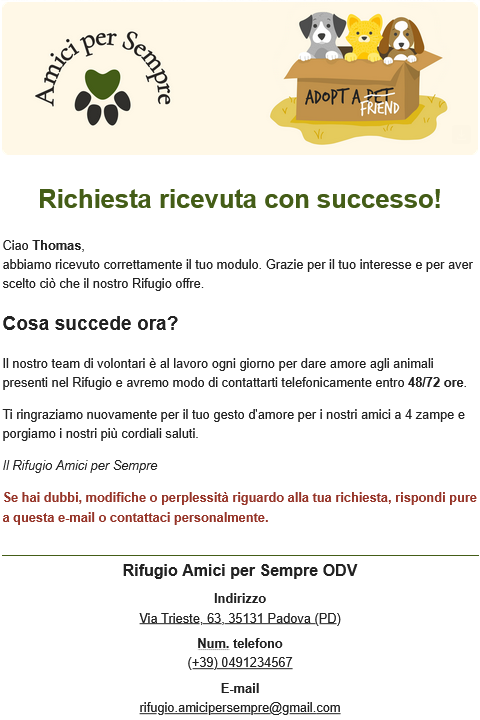
\includegraphics[width=\linewidth]{../Resources/Images/email-rifugio.png}
			\end{minipage}
		\end{citabox}
	\end{itemize}
	\subsubsection{Composer (\texttt{vendor})}
	È stato fatto uso di Composer come programma applicativo per l'installazione delle librerie necessarie all'interno del progetto di \textbf{Emogrifier} (CSS inline parser) e \textbf{PHPMailer} (composizione automatica dell'email). Questa scelta permette la scalabilità del progetto, in quanto risulta semplice l'integrazione di nuove librerie senza l'obbligo di scaricarle manualmente, e la delegazione del compito di gestione delle dipendenze tra, per l'appunto, librerie.
	\subsubsection{\texttt{db-access.php}}
	File PHP per la gestione dell'apertura e chiusura della connessione alla base di dati. Lo script implementa le funzioni di apertura, chiusura e restituzione della connessione, insieme alla funzione di esecuzione della query che ha il compito di gestirne i parametri in ingresso, preparare lo statement e renderlo innocuo a \textbf{SQL Injection} e restituire uno/più risultati in base alla tipologia (SELECT, UPDATE, DELETE) della query.
	\subsubsection{\texttt{.htaccess}}
	Il seguente file permette le operazioni di rooting del sito web. Nello specifico permette:
	\begin{itemize}
		\item visualizzazione delle pagine di errore personalizzate al posto della schermata predefinita del server per gli errori \texttt{500} e \texttt{404};
		\item \textbf{pulizia dell'URL} di pagina con rimozione dell'estensione \texttt{.php};
		\item definizione dell'\textbf{albero delle pagine}, come descritto dall'elemento breadcrumb, senza possibilità di visualizzare i percorsi interni al repository di progetto.
	\end{itemize}
	\subsection{\texttt{pannello-filtri.php}}
	Il seguente file contiene al suo interno una dichiarazione modulabile del pannello filtri utilizzato all'interno delle pagine di adotta, gestione dei ticket e gestione delle richieste per portare in adozione un'animale. Questo strumento permette di filtrare le liste di elementi grazie a campi di ricerca personalizzabili per ciascuna pagina, in base alle informazioni che si possono ottenere durante la navigazione. La modularità di questo elemento permette, per l'appunto di essere riutilizzato in più pagine, con una gestione centralizzata del popolamento dei campi e dell'URL di ricerca, il quale deve contenere i criteri per il filtraggio dei risultati, inviati al server in modalità GET.
	\subsection{Base di dati}
	Per il corretto funzionamento del sito web è stata implementata una base di dati in linguaggio MySQL all'interno del \textbf{RDBMS Maria DB}, la quale presenta al suo interno tutte le entità fondamentali per gestire le richieste degli utenti per l'adozione degli animali e la possibilità di portarli in adozione al rifugio; il tutto può essere centralizzato per l'amministratore tramite gestione delle richieste, una volta programmate, in calendario.
	\begin{figure}[h!]
		\centering
		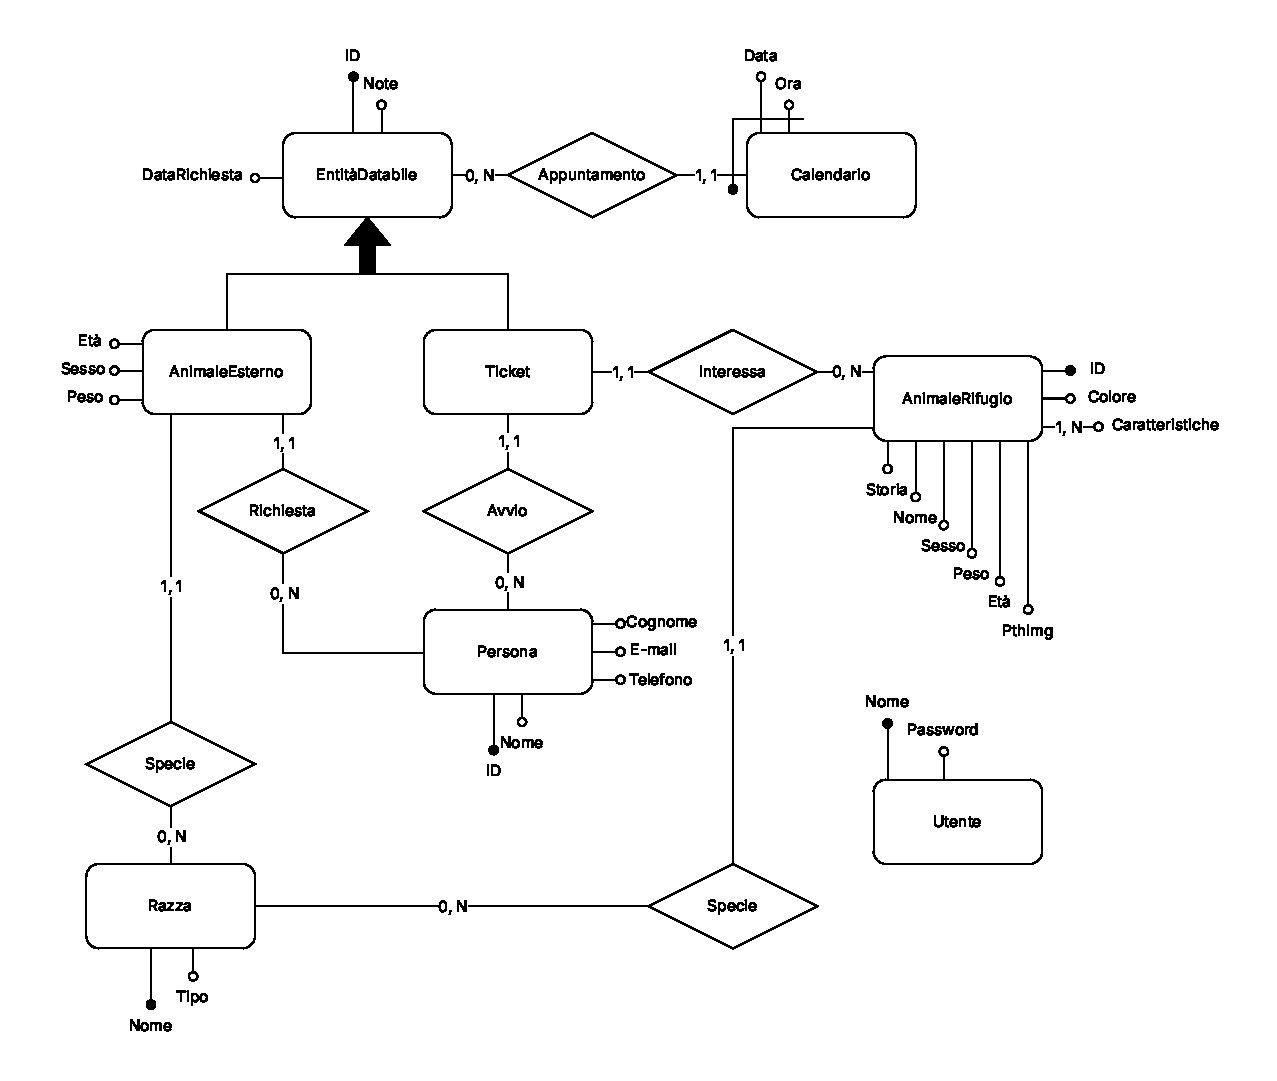
\includegraphics[scale=0.75]{../Database/er-rifugio.pdf}
		\caption{Diagramma ER della base di dati}
	\end{figure}\\
	Per questioni di spazio, ma volendo comunque approfondire il diagramma soprariportato, si evidenziano le seguenti scelte progettuali:
	\begin{itemize}
		\item l'entità \texttt{EntitàDatabile} viene utilizzata per accorpare gli attributi comuni di \texttt{AnimaleEsterno} e \texttt{Ticket}, ovvero la richiesta di adozione; in particolare l'entità serve per permettere di calendarizzare le tuple, delle tabelle distinte, all'interno dell'entità \texttt{Calendario}, potendo usare ID univoco;
		\item l'entità \texttt{Utente} presenta un campo Password criptato tramite funzione di hashing \texttt{bcrypt} basata su cifratura Blowfish;
		\item l'entità \texttt{Razza} presenta un campo Lingua che viene utilizzato per popolare l'attributo \texttt{lang} HTML e poter quindi rendere accessibile la pronuncia di una razza nel momento in cui viene utilizzata all'interno del sito;
		\item l'entità \texttt{AnimaleRifugio} presenta il campo Età di tipo \texttt{FLOAT(2, 2)}, permettendo così di estrapolare dalle cifre unitarie gli anni dell'animali, mentre da quelle decimali i mesi di quest'ultimo; questa scelta permette di filtrare anche per mesi gli animali del Rifugio.
	\end{itemize}
	Una copia del DUMP per la base di dati è presente al percorso interno di progetto \texttt{Database/dump-rifugio.sql}
	\subsection{Sicurezza}
	Per quanto concerne la sicurezza del sito web sono state applicate le seguenti tecniche di prevenzione danni nei confronti delle tecnologie client/server-side:
	\begin{itemize}
		\item creazione, come già parlato precedentemente, della funzione \texttt{exeQuery} la quale fa uso di \texttt{mysqli\_prepare()} per parametrizzare le query e trattare l'input, eccetto dati integer/double, come una semplice stringa; ciò previene \textbf{SQL Injection};
		\item password dell'amministratore salvata con tecnica di criptazione tramite funzione di hashing \texttt{bcrypt} basata su cifratura Blowfish;
		\item protezione da attacchi di tipo \textbf{XSS (Cross-Site Scripting)} grazie alla funzione \texttt{htmlspecialchars()} inserita all'interno di ogni funzione per l'estrapolazione dei dati dal database ed evitare l'inserimento di elementi HTML che potrebbero rompere la struttura della pagina.
	\end{itemize}
	\section{Accessibilità e usabilità}
	Uno degli aspetti fondamentali nella progettazione web risulta essere l'attenzione all'accessibilità, ovvero il ramo che si occupa di rendere utilizzabile un sito web da chiunque. Per questo progetto si è fatto riferimento allo standard \textbf{WCAG (Web Content Accessibility Guidelines) 2.2}, inclusivo dello standard 2.1.
	\subsection{Elementi fondamentali}
	L'accessibilità all'interno di questo progetto si concretizza nel rispetto di regole ben specifiche dello standard sopracitato:
	\begin{itemize}
		\item separazione netta tra livello di struttura (HTML5), presentazione (CSS3) e comportamento (JavaScript); questo permette di incorporare elementi di arricchimento delle pagine senza rompere la struttura solida alla base;
		\item utilizzo di file HTML semantici e validati, per garantire che non si "rompano" alla visualizzazione, rovinando così la lettura tramite tecnologie assistive;
		\item rispetto della norma WCAG 2.5.8, in quanto tutti gli elementi cliccabili interni al sito presentano un'area cliccabile di almeno \texttt{24x24} pixel garantendo il livello minimo AA; i pulsanti, invece, garantiscono un livello di accessibilità AAA con una dimensione minima di \texttt{44x44} pixel;
		\item utilizzo di unità relative all'interno dei fogli di stile per garantire il ridimensionamento degli elementi in base alle necessità dell'utente;
		\item implementazione di funzionalità "\textbf{rimuovi sfondo}", permettendo ad un utente con difficoltà visive o ADHD di concentrarsi più facilmente nella lettura del testo;
		\item implementazione di funzionalità "\textbf{tema chiaro/scuro}", permettendo ad utenti ipovedenti (affetti da fotosensibilità, patologie dell'occhio, ...) di navigare il sito con minore difficoltà;
		\begin{quote}
			\textbf{NB} Queste ultime due funzionalità vengono rese fruibili anche tramite screen reader, in quanto utili agli utenti ipovedenti per le ragioni soprariportate.
		\end{quote}
		\item utilizzo di animazioni con un tempo di esecuzione minimo pari a \texttt{0.3}s per non inficiare sull'attenzione dell'utente.
		\item è stato fatto uso di un font accessibile quale \href{https://fonts.google.com/specimen/Inter?query=inter}{\texttt{Inter}}, privo di grazie per rendere la lettura delle pagine facile a qualsiasi utente e preservare un estetica pulita;
		\item validazione dei campi di un form sia a livello \textbf{client-side} che \textbf{server-side}, con particolare attenzione alla stampa degli errori commessi dall'utente, i quali vengono annunciati per essere subito compresi anche da un utente che naviga con tecnologie assistive;
		\item inserimento di attributi \texttt{lang} per l'identificazione della lingua dell'elemento e permettere una lettura efficace da parte dello screen-reader.
	\end{itemize}
	\subsection{Orientamento e navigazione}
	Per quanto riguarda questa sezione si elencano le best practices adottate per rendere il sito web di facile navigazione:
	\begin{itemize}
		\item utilizzo dell'elemento breadcrumb, il quale permette all'utente di orientarsi all'interno del sito web;
		\item implementazione di un pulsante "torna in cima", per facilitare il ritorno alla parte superiore della pagina;
		\item header e elementi di selezione del contenuto (pannello filtri, pannello di gestione calendario) definiti \texttt{sticky} per permetterne la reperibilità durante la navigazione;
		\item utilizzo di tag \texttt{<details>} per la visualizzazione di informazioni principali all'interno di \texttt{summary} e dettagli ad esso collegati nella seziona a scomparsa; ciò permette all'utente di navigare con semplicità senza l'obbligo di lettura, soprattutto con screen reader, di un contenuto potenzialmente non richiesto dall'utente stesso;
		\item elemento di notifica toast, con focus e role \texttt{alert} per avvisare l'utente al successo o meno di un'azione interna al sito (es. calendarizzazione di un appuntamento);
		\item testing ed eventuale correzione della navigazione da tastiera tramite pulsante Tab, con possibile esclusione di alcuni elementi aventi \texttt{tabindex=-1}, altrimenti difficili da navigare (es. Google map nella homepage del sito).
	\end{itemize}
	\subsection{WAI-ARIA}
	Un ulteriore pratica adottata all'interno del sito web per renderlo accessibile è l'utilizzo di specifiche WAI-ARIA (Web Accessibility Initiative - Accessible Rich Internet Applications) per definire ruoli e proprietà aggiuntive per rendere la navigazione tramite tecnologie assistive il più comprensibile possibile. Alcuni degli attributi utilizzati sono:
	\begin{itemize}
		\item \texttt{aria-label} per la definizione dell'etichetta di pulsanti e renderli così più comprensivi nel loro scopo;
		\item \texttt{aria-hidden} per nascondere elementi, come icone vettoriali, che altrimenti verrebbero percepite dallo screen reader;
		\item \texttt{aria-labelledby} per fornire un titolo significativo a ciascun tag \texttt{<section>} all'interno del sito web;
		\item \texttt{aria-expanded} per far comprendere ad un utente ipovedente/non vedente se un elemento si è espanso o meno;
		\item \texttt{aria-live} per avvertire l'utente nel momento in cui il contenuto di un elemento è cambiato dopo una determinata azione;
		\item attributo \texttt{role} per la definizione del ruolo di ciascun elemento e di come debba essere interpretato dalla tecnologia assistiva.
	\end{itemize}
	\subsection{Colori e Brand Identity}
	Per quanto concerne l'utilizzo dei colori, quindi di una palette unificata, si è voluto far fronte sia ad un'esigenza estetica che funzionale/accessibile. Nello specifico la palette richiama quelli che sono i colori principali per un'attività a stretto contatto con gli animali, rispettando al tempo stesso quelle che sono le necessità minime di \textbf{contrasto AA (valore 4.5:1)} richieste all'interno dello standard WCAG 2.2. Si riportano di seguito le palette utilizzate con i relativi contrasti.\vspace{3cm}
	\begin{figure}[h!]
		\centering
		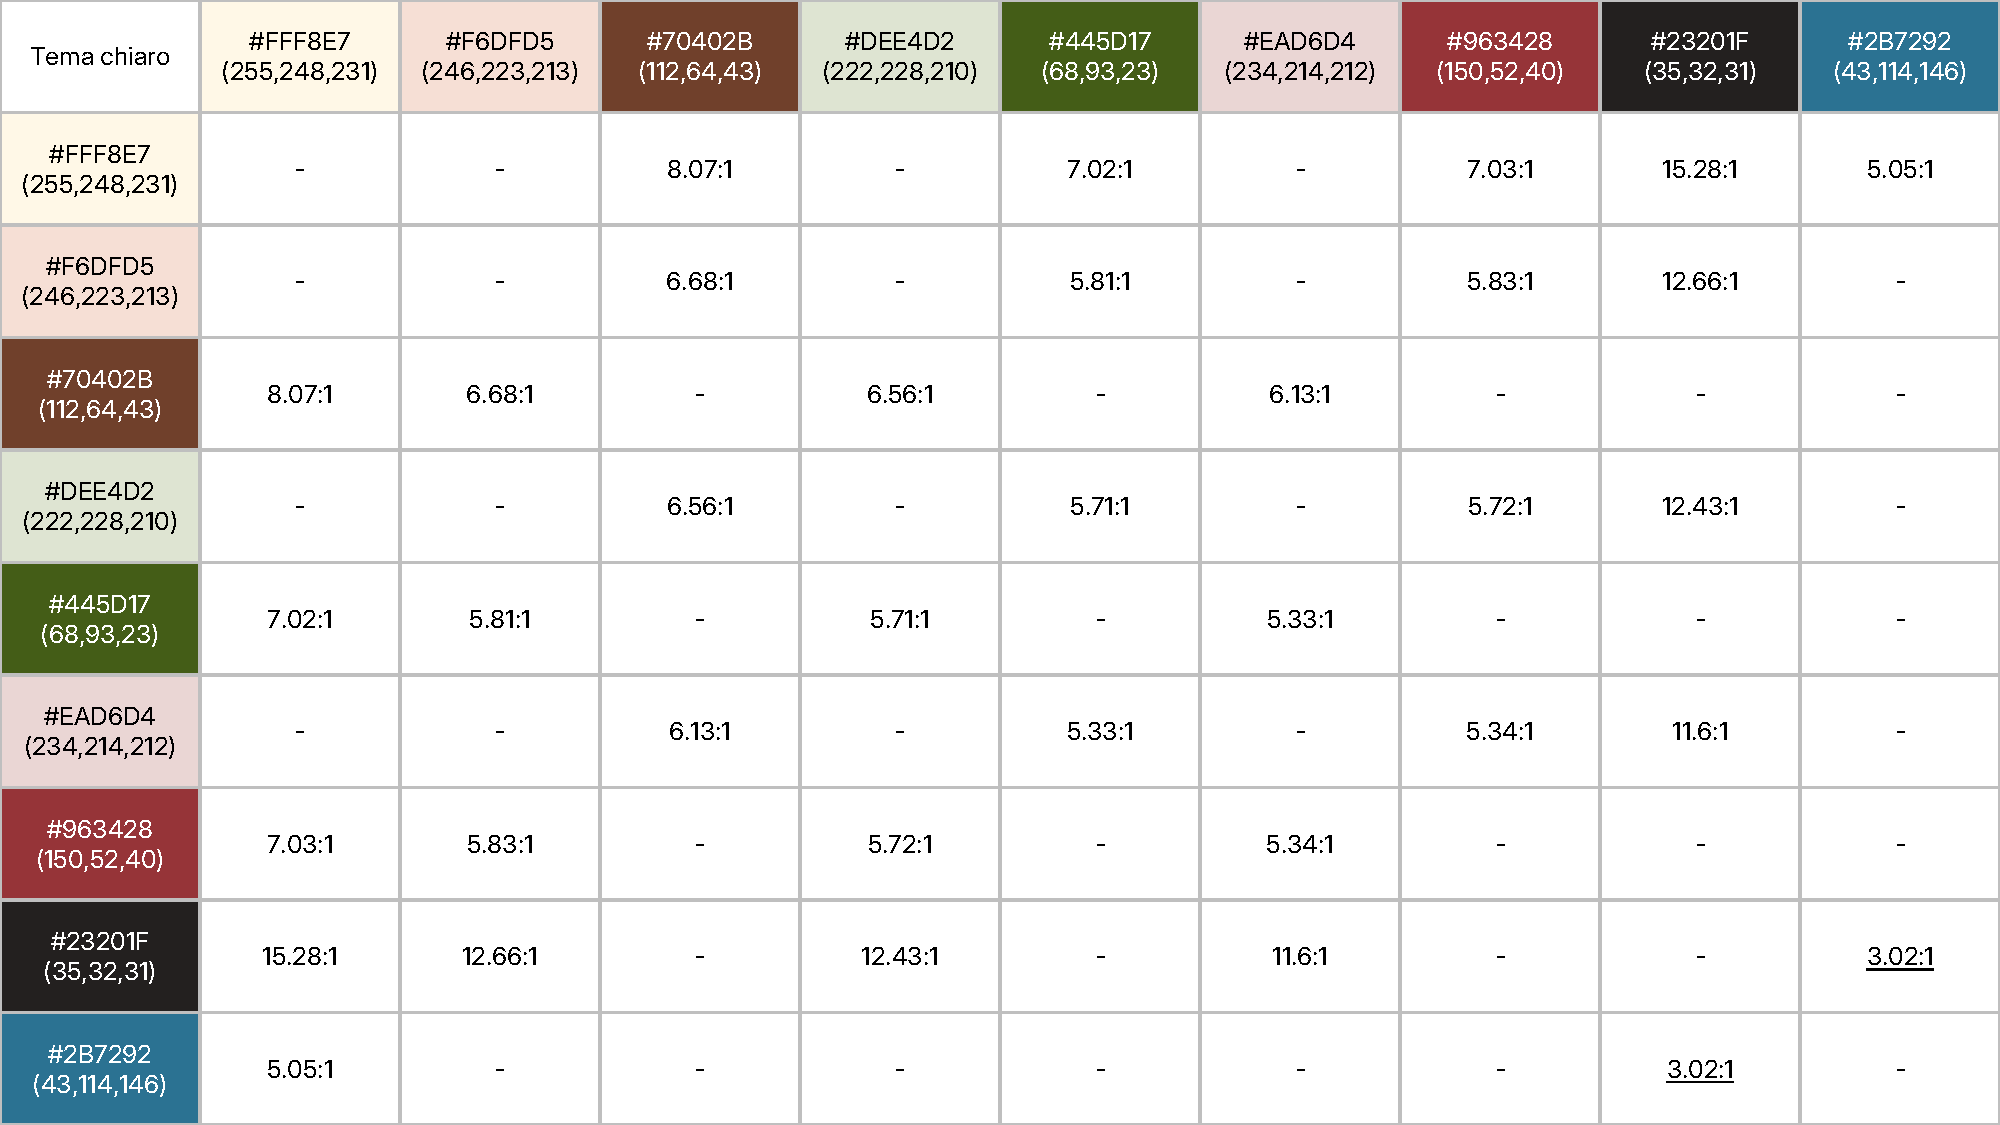
\includegraphics[scale=0.3]{../Design/tema-chiaro.pdf}
		\caption{Tema chiaro}
	\end{figure}
	\begin{figure}[h!]
		\centering
		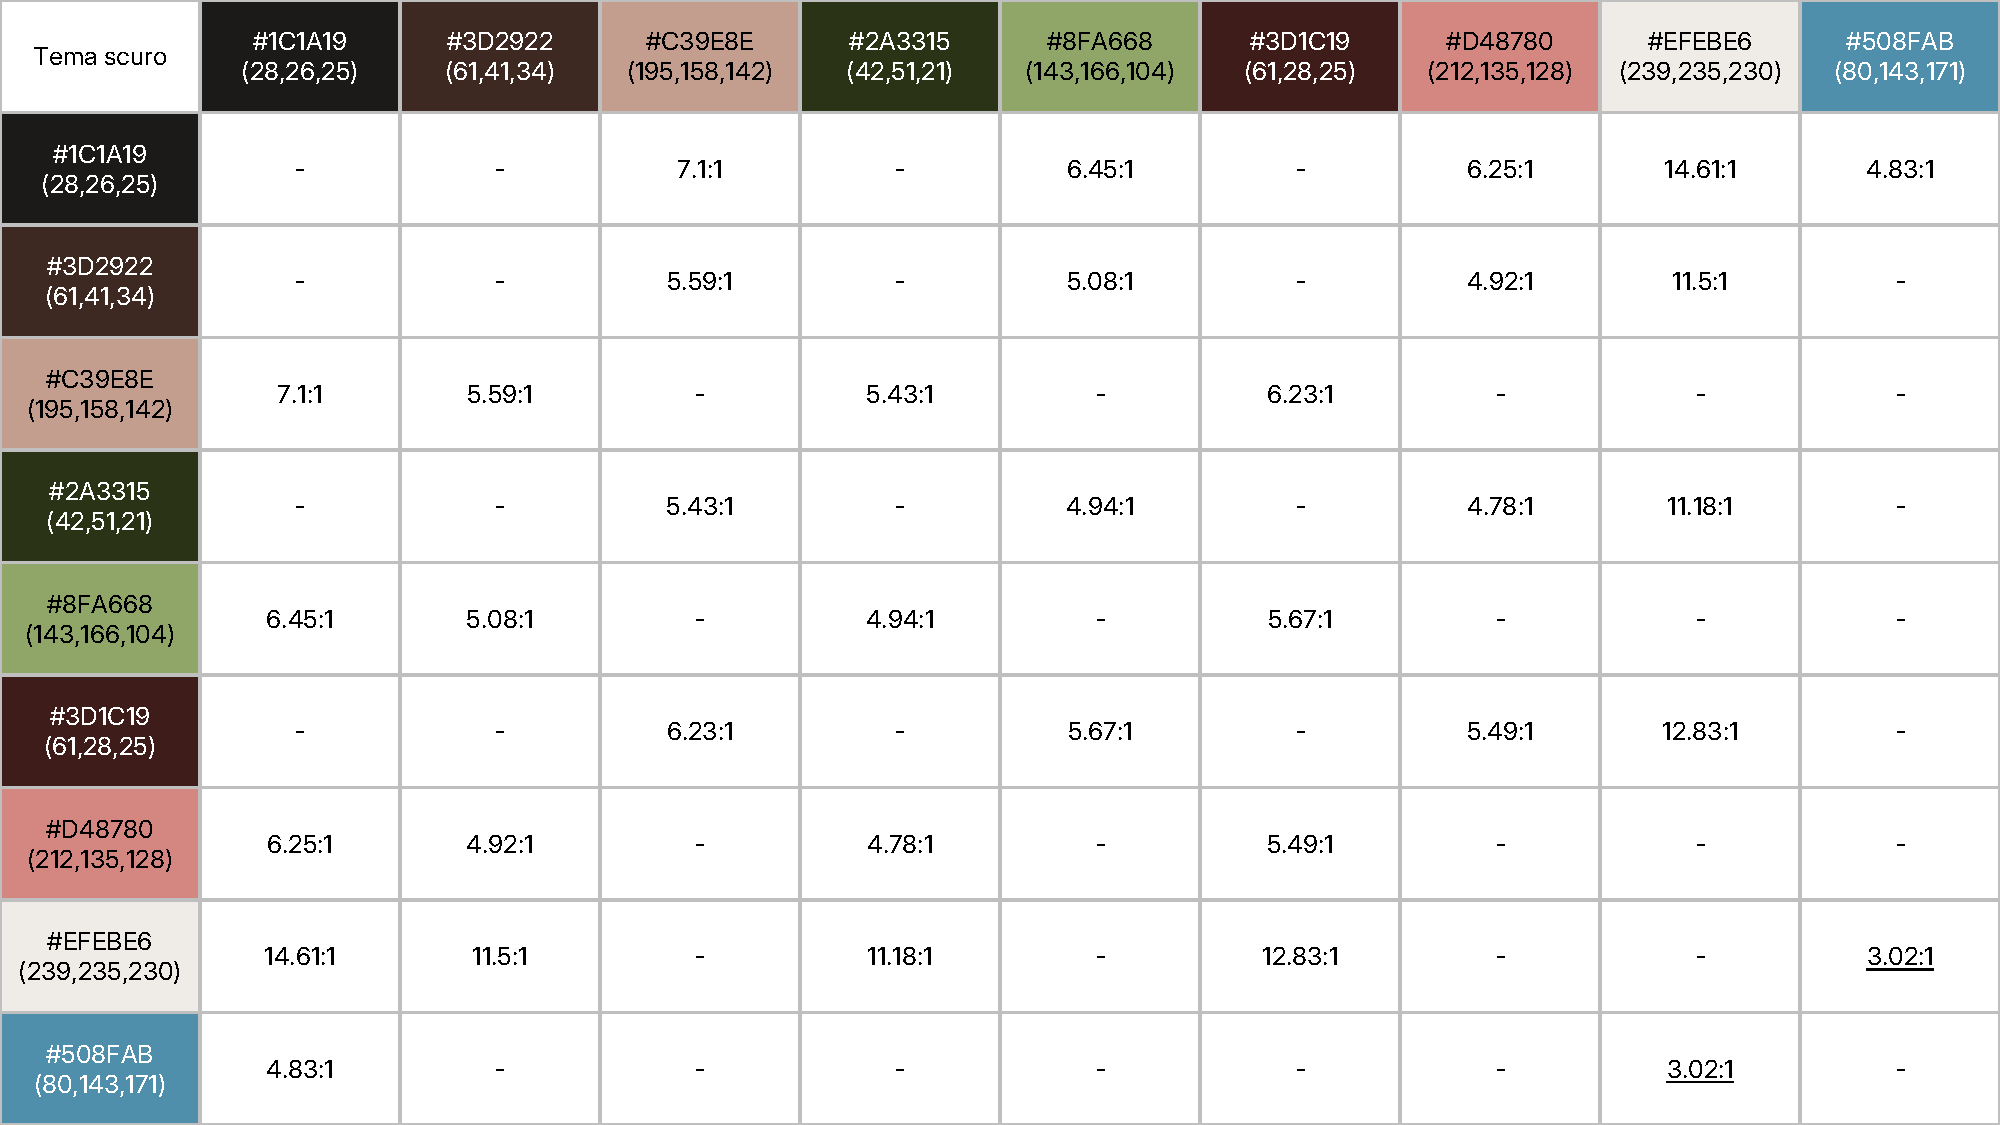
\includegraphics[scale=0.3]{../Design/tema-scuro.pdf}
		\caption{Tema scuro}
	\end{figure}\\
	Com'è possibile notare dalle tabelle soprariportate tutti i contrasti rispettano ciò che è stato descritto nel paragrafo precedente. È stato riportato, all'interno delle tabelle, anche il contrasto tra il colore per i link non visitati (\texttt{\#2B7292} e \texttt{\#508FAB}) e il testo normale (\texttt{\#23201F} e \texttt{\#EFEBE6}), che è il colore dei link già visitati, che è pari a 3.02:1, sufficiente per comprenderne la differenza. Si vuole evidenziare, inoltre, che per l'ideazione del tema scuro non c'è stata una semplice "inversione" dei colori, ma bensì uno studio che garantisse una \textbf{desaturazione} dei colori luminosi, come testo o bordi, in quanto, a differenza del tema chiaro, i colori chiari hanno una luminosità differente rispetto a quelli scuri, tendendo così a risaltare maggiormente in constrasto con uno sfondo quasi nero. Tutti i colori riportati all'interno di queste palette aiutano a creare così una \textbf{brand identity} per il sito che diventa riconoscibile nella sua grafica e tonalità.
	\subsection{Convenzioni interne del sito}
	Per aiutare l'utente durante la navigazione all'interno del sito si è fatto uso delle seguenti convenzioni interne:
	\begin{itemize}
		\item \textbf{colori di pulsanti}, compreso di quest'ultimi sfondo, bordo e testo, sono stati standardizzati con le tonalità del verde, per essere immediatamente identificabili in quanto elementi cliccabili;
		\item i \textbf{link non visitati} presentano colore azzurro, a differenza di quelli visitati che si "nascondono" riprendendo il colore del testo; entrambi rimangono comunque sottolineati per identificazione immediata da parte dell'utente;
		\item i \textbf{link che portano a pagine esterne} dal sito vengono segnalati tramite l'uso di un'icona standard nella progettazione web che riporta una freccia che punta verso l'esterno di un quadrato.
	\end{itemize}
	\section{Test e validazione}
	Sono stati eseguiti vari test per garantire l'accessibilità del sito e per validare il codice. Di seguito la lista di strumenti che sono stati utilizzati per automizzare alcuni test:
	\begin{itemize}
		\item \textbf{W3C Validator:} sturmento che ci ha permesso di analizzare il codice html di ogni pagina per garantire che fosse sotto gli standard di W3C.
		\item \textbf{WAVE Evaluation Tool:} estensione disponibile al browser che ha analizzato la pagina direttamente sotto gli standard alle linee guida di WCAG 2.2.
		\item \textbf{WebAIM Contrast Checker:} strumento utilizzato per verificare il contrasto tra i colori utilizzati nel progetto, garantendo il rispetto del livello di accessibilità AA.
	\end{itemize}
	Inoltre, durante la fase dello sviluppo del codice sono stati eseguiti vari test manuali per garantire tutti gli aspetti di accessibilità e funzionalità che non possono essere testati automaticamente:
	\begin{itemize}
		\item \textbf{Test con NVDA:} tutte le pagine sono state testate e strutturate correttamente in modo da garantire il giusto funzionamento dello screen reader NVDA. In particolare:
		\begin{enumerate}
			\item I flag di conteggio nel pannello filtri hanno l'attributo "aria-live=polite" per permette allo screen reader di non fermarsi se il numero si aggiorna dinamicamente mentre sta leggendo la pagina.
			\item Nel pannello filtri per ogni bottone di sezione è stato aggiunto l'attributo "aria-describedby" per informare l'utente di quanti filtri sono stati modificati in quella sezione.
			\item Sono stati inseriti "aria-hidden" per gli elementi che non devono essere letti.
			\item Per le immagini già corredate da figcaption, l'attributo "alt" è stato lasciato vuoto (alt="") per evitare che lo screen reader fornisca una descrizione ridondante o poco rilevante dal punto di vista contestuale.
			\item Ogni termine non italiano è stato marcato con l'attributo "lang".
		\end{enumerate}
		\item \textbf{Supporto per tastiera:} si ha prestato attenzione per rendere il sito navigabile da tastiera. Ogni elemento interagibile può essere selezionato senza l'utilizzo di mouse, in particolare:
		\begin{enumerate}
			\item Ogni elemento dei form ha corretto label associato utilizzando gli attributi "for" nelle label ed "aria-labelledby" nel caso dei gruppi checkbox nel pannello filtri e la barra di ricerca nelle pagine di amministrazione.
			\item I radio button e checkbox sono stati raggruppati correttamente in fieldset con eventuale legenda per descrivere il gruppo.
			\item In Ogni campo obbligatorio è stato aggiunto l'attributo "aria-describedby" per avvisare l'utente di eventuali errori nella compilazione dei form in modo dinamico.
			\item Il "tabindex" del pannello filtri e delle relative sezioni è stato modificato per prevenire la navigazione da tastiera quando questi sono chiusi e non visibili.
		\end{enumerate}
		\item \textbf{Compatibilità browser multipli:} si ha verificato che il sito fosse correttamente renderizzato ed utilizzabile dai principali browser (Edge, Firefox, Chrome, Brave, Safari),
		\item \textbf{Compatibilità browser da telefono:} si ha verificato che il sito fosse correttamente renderizzato ed utilizzabile da dispositivi mobili.
		\item \textbf{Test di reindirizzamento delle pagine:} si ha testato il corretto funzionamento dei reindirizzamenti configurati in .htaccess, sia nella navigazione generale che nelle relative pagine di errore.
		\item \textbf{Test del layout di stampa:} si ha verificato che durante la stampa la maggior parte dei bottoni venissero nascosti e che non ci fossero elementi tagliati dal cambio di pagina.
		\item \textbf{Test di funzionalità senza Javascript:} alcuni componenti usufruiscono di codice a lato client per rendere l'esperienza più fluida e animata: in quel caso si ha verificato che il sito funzionasse senza aver bisogno di codice Javascript. In particolare:
		\begin{itemize}
			\item Ogni campo dei form deve essere verificato sia da lato client con Javascript che da lato server con PHP, rendendo quindi il primo solo un controllo aggiuntivo e non essenziale.
			\item Il pannello filtri deve essere nascosto di default, e mostrato solamente se il codice Javascript è attivo, in modo da evitare una esperienza utente incompleta.
			\item Il form di porta in adozione deve sostituire il select per la selezione della razza con un input normale, elencando sotto le razze disponibili nel database. La razza inserita sarà effettivamente controllata dal php a lato server.
		\end{itemize}
		\item \textbf{Test funzionali:} sono stati eseguiti vari test per controllare le seguenti funzionalità:
		\begin{enumerate}
			\item \textbf{Invio e-mail di conferma:} quando l'utente invia un form di adozione o di richiesta porta in adozione, il sistema deve inviare una e-mail di conferma all'indirizzo specificato, con le corrette informazioni e il layout CSS definito dal file style-email.css
			\item \textbf{Pagina di amministrazione:} la pagina deve indicare a chi accede quante richieste devo essere gestite per entrambi i tipi (adozione / porta in adozione), e quanti appuntamenti sono programmati per quel giorno.
			\item \textbf{Pagine di gestione richieste:} devono essere mostrate nella lista tutte le richieste che non sono state datate nel calendario, e tutte le richieste già assegnate nel calendario che sono previste per una data / ora futura. In particolare:
			\begin{enumerate}
				\item Nella \textbf{gestione ticket} (richieste di adozione), devono essere mostrati tutti gli animali disponibili nel centro di adozione. Per ogni animale il sistema deve indicare quante richieste sono da gestire, e quali sono invece già gestite.
				\item Nella \textbf{gestione richieste inserimento animali in rifugio} invece, devono essere mostrati tutti gli animali "esterni" al rifugio, con aggiuntivo descrittore che indica se la richiesta è stata gestita o no.
			\end{enumerate}
			Inoltre, ogni richiesta deve essere popolata correttamente dal database (con eventuale immagine dell'animale) e gestita correttamente da tre funzionalità principali:
			\begin{enumerate}
				\item Il pulsante \emph{info} deve aprire un dialog popup che informa di eventuali note della richiesta.
				\item Il pulsante \emph{assegnazione a calendario} deve aprire un dialog popup che consenta di selezionare data e ora valide per programmare la visita (con "valide" si intende una data non passata e dentro l'orario lavorativo del centro).
				\item Il pulsante \emph{eliminazione} deve aprire un dialog popup che richieda la conferma dell'azione e rimuovi la richiesta dal database.
			\end{enumerate}
			Se la richiesta è già gestita, i pulsanti (b) e (c) vengono sostituiti da un pulsante che porta al calendario in cui la visita è stata programmata.
			\item \textbf{Calendario:} la pagina deve essere popolata correttamente dal database, e deve essere possibile navigare tra settimane / mesi. Ogni richiesta deve avere:
			\begin{enumerate}
				\item Il pulsante \emph{info} con funzione identica a quella citata sopra.
				\item Il pulsante \emph{modifica appuntamento} che deve aprire un dialog popup per modificare la data e l'ora della visita (ovviamente data e ora valide)
				\item Il pulsante \emph{eliminazione} che deve aprire un dialog popup per la conferma della rimozione da calendario (rendendo la richiesta nuovamente da gestire nelle pagine di gestione richieste).
			\end{enumerate}
			In caso di data passata l'utente potrà solo verificare le note della prenotazione.
			\item \textbf{Pannello filtri:} il pannello deve soddisfare le seguenti funzionalità:
			\begin{itemize}
				\item Se l'accesso avviene tramite desktop il pannello può essere aperto al lato destro della pagina.
				\item Se l'accesso avviene tramite dispositivo mobile il pannello può essere aperto come dialog popup.
				\item Il pannello deve cambiare il numero di filtri selezionati dinamicamente, sia in maniera generale (dal bottone di "applica filtri"), che per ogni sezione (flag di conteggio). 
				\item Se il pannello è stato aperto laterlamente deve essere già aperto al caricamento della pagina. 
				\item I campi vuoti del form del pannello devono essere omessi dalla richiesta GET.
				\item I filtri devono essere applicati correttamente nelle pagine che usufruiscono del pannello. 
				\item Anche se il pannello filtri e la barra di ricerca sono in form separati, la richiesta deve poter tenere eventuali parametri GET già presenti nell'url per evitare la perdita di filtri durante la ricerca e viceversa.
			\end{itemize}
			\item \textbf{Pagina di adozione:} La pagina deve essere popolata correttamente dal database, e ogni scheda deve portare alla pagina dell'animale selezionato.
			\item \textbf{Scheda animale:} La pagina deve essere popolata correttamente dal database.
			\item \textbf{Pagina di porta in adozione:} Il select della razza nel form di richiesta deve popolarsi in modo dinamico in base al tipo di animale scelto tramite richiesta ajax alla pagina razze-json.php
			\item \textbf{Accesso amministratore:} In caso si navigasse nella pagina di accesso quando si ha già eseguito il login, il sito deve invece mostrare la pagina di logout.
			\item \textbf{Pagine di amministrazione:} Se l'utente prova ad entrare nelle pagine di amminstrazione senza effettuare il login, deve essere reindirizzato alla pagina di errore 401.
		\end{enumerate}
	\end{itemize}
	\section{SEO e prestazioni}
	Il ranking del sito web, specialmente per quanto riguarda un'attività no-profit e geograficamente circoscritta come il Rifugio in oggetto, è un aspetto fonamentale. Per questo ci si basa sull'incremento della SEO (Search Engine Optimization) per fare in modo che il sito venga proposto ai livelli più alti possibili della \textbf{SERP (Search Engine Results Page)}. Le best practices più comuni adottate in questo progetto sono:
	\begin{itemize}
		\item separazione tra struttura (HTML5), presentazione (CSS3) e comportamento (JavaScript) per permettere un caricamento rapido delle pagine del sito.
		\begin{quote}
			\textbf{NB} Tramite estensione \textbf{Chrome Browser \href{https://chromewebstore.google.com/detail/lighthouse/blipmdconlkpinefehnmjammfjpmpbjk?hl=it}{Lighthouse}} è stato possibile verificare una velocità di caricamento della pagina ottimo (99/100), con una velocità di caricamento massima pari a 0.5s.
		\end{quote}
		\item uso di formati leggeri per le immagini del sito, come \texttt{.jpg} o \texttt{WebP};
		\begin{quote}
			\textbf{NB} Le immagini all'interno della sezione esperti della homepage del sito, rispettivamente gli operatori e gli istruttori ENCI sono state generate con l'utilizzo di Intelligenza Artificiale.
		\end{quote}
		\item inserimento di keywords e metadati dinamici all'interno delle diverse pagine tramite scripting PHP;
		\item breadcrumb e link di navigazione del sito per permettere agli algoritmi di ispezione delle pagine di analizzare più pagine possibili del sito web;
		\item uso di tag \texttt{<strong>} ed \texttt{<em>} per la marcatura delle keywords all'interno del sito;
		\item metatag con attributo \texttt{property="og:..."} per definire parametri utili nella fase di condivisione del sito tramite socials, come logo, descrizione, ...;
		\item ottimizzazione del \textbf{layout responsive} per permettere agli algoritmi di ispezione di alzare il livello di ranking;
		\item tag \texttt{<title>} con lunghezza inferiore ai 55 caratteri, dallo specifico al generale e univoco per ciascuna pagina;
		\item uso di metatag \texttt{description} dinamico per ciascuna pagina, il quale non massimizza direttamente il ranking ma potrebbe aiutare nel \textbf{CTR (Click-Through Rate)} aumentando così il numero di interazioni che gli utenti hanno con il sito web;
		\item dichiarazione degli elementi grafici vettoriali all'interno del file \texttt{icons.svg}, la quale scelta permette di diminuire la velocità di caricamento della pagina, permettendo al browser di caricare in un momento unico tutte le icone di cui il sito ha necessità; il vantaggio risiede anche nella manipolazione del colore e nell'organizzazione delle suddette icone vettoriali;
		\item utilizzo di tag \texttt{<h1>} univoco per pagina (logo del sito) contenente la keyword principale, abbinato all'uso gerarchico dei tag \texttt{<h2>...<h6>};
		\item link ai \textbf{social media} del Rifugio, anche se non concretamente presenti si evidenzia che aiutano come elemento per la SEO; concetto analogo è valido anche per l'indirizzo fisico del Rifugio, il quale aiuta alla connessione con ricerche in Google Maps.
	\end{itemize}
	Si è deciso inoltre di lavorare sulla SEO semantica, ampliando così il quantitativo di scelte architetturali adottate per l'ottimizzazione del ranking. Di seguito viene riportata la descrizione dei file cardine. Nello specifico è stato implementato il vocabolario semantico \texttt{Schema.org} attravero il formato \textbf{JSON-LD (JavaScript Object Notation for Linked Data)}, utilizzato per inserire dati strutturati in formato JSON all'interno delle pagine web e renderli facilmente ispezionabili dagli algoritmi di ranking.
	\subsection{\texttt{faq-schema.js}}
	File "iniettabile" all'interno della homepage, la quale al suo interno presenta \textbf{FAQs (Frequently Asked Questions)} per approfondire eventuali dubbi da parte dell'utente. Lo \texttt{Schema.org} in questione si pone l'obiettivo di rendere disponibili ai crawler le domande e le risposte contenute all'interno della pagina, strutturate e leggibili facilmente. Questa sezione aiuta ad aumentare il ranking, in quanto ha la possibilità di abbinare criteri di ricerca generali dell'utente (eseguiti nella barra di ricerca del browser) alla pagina del Rifugio, tramite per l'appunto risposte ad eventuali domande.
	\subsection{\texttt{org-schema.js}}
	Questo secondo file viene "iniettato" all'interno della homepage, pagina di adotta, pagina di porta in adozione e scheda animale. In questo contesto il file permette di comunicare in modo univoco al browser quelli che sono i dati principali dell'ente, i quali ne identificano l'identità. Alcuni degli attributi definiti nello schema sono: tipologia ente specifica per rifugio animali (\texttt{AnimalShelter}), telefono, email, localizzazione geografica, orari di apertura e scopo di lucro dell'ente (\texttt{\$} ovvero no-profit). Eventualmente è stata aggiunta la possibilità di collegamento ai link social anche se non presenti nel concreto. Questi dati aiutano a creare autorevolezza per l'ente del Rifugio, permettendo così una massimizzazione del ranking all'interno della SERP.
	\section{Organizzazione del lavoro}
	Ogni membro ha contribuito alla progettazione del database e alla scelta dei colori utilizzati nel sito, valutati in base al contrasto secondo gli standard delle linee guida WCAG 2.2, con Thomas Morettin come principale contributore in questo ambito.
	Per quanto riguarda lo sviluppo delle pagine, il gruppo si è organizzato per la realizzazione del progetto suddividendo il lavoro in base alle pagine da realizzare, ognuna delle quali prevedeva lo sviluppo di HTML, CSS, PHP e JavaScript:
	\begin{itemize}
		\item Thomas Morettin: header e footer, pagina \emph{Index}, pagina \emph{Calendario}, pagina \emph{Gestione ticket}, pagina \emph{Amministrazione}.
		\item Felician Mario Necsulescu: pagina \emph{Adotta}, pagina \emph{Scheda animale}, pagine di \emph{Errore}.
		\item Niccolò Feltrin: pagina \emph{Accesso}, pagina \emph{Porta in adozione}, pagina \emph{Gestione richieste inserimento rifugio} 
	\end{itemize}
	A livello funzionale, sono state assegnate:
	\begin{itemize}
		\item a Thomas Morettin il sistema di invio e-mail.
		\item a Niccolò Feltrin il pannello filtri utilizzabile modularmente.
		\item a Felician Mario Necsulescu la maggior parte della validazione dei campi nei form presento nel sito.
	\end{itemize}
	Si è data quindi la responsabilità ad ogni membro del gruppo di validare l'accessibilità delle proprie pagine e di testarne il corretto funzionamento.
	\section{Conclusioni e difficoltà incontrate}
	In conclusione, il sito è stato progettato in un contesto il più possibile realistico, con l'obiettivo di sviluppare un sistema in grado di gestire in modo completo tutte le transazioni (adozioni e appuntamenti) di un centro di adozione immaginario. Particolare attenzione è stata posta affinché il sistema risultasse accattivante, accessibile, semplice da utilizzare, immediato e distintivo.
	Il progetto ci ha permesso di esplorare diverse fasi dello sviluppo web, dalla progettazione del logo alla definizione delle funzionalità principali del sito, offrendo un'esperienza completa e pratica che ha arricchito le competenze di tutti i membri, sia sul design pulito e funzionale, sia sulla realizzazione di un servizio web operativo.
	L'attività ha inoltre fornito l'opportunità di gestire efficacemente il lavoro di gruppo, sperimentando la suddivisione dei compiti e l'organizzazione delle pagine. Particolarmente significativa è stata la progettazione di un sistema modulare per la creazione delle pagine e l'implementazione di un meccanismo di invio automatico delle e-mail, che ha consentito di rendere il sito più completo e professionale.
	Grazie alla sua struttura modulare, il progetto può essere facilmente esteso e adattato per un'implementazione reale in un centro di adozione, offrendo così un'esperienza arricchente per i membri del gruppo.
	
	\vspace{0.5cm}

	Alcune difficoltà sono state riscontrate durante la progettazione del sito:
	\begin{itemize}
		\item \textbf{Accessibilità:} in alcune funzionalità del sito, come nelle pagine di gestione delle richieste, nelle schede animali o nel pannello dei filtri, è stato particolarmente impegnativo cercare di trovare un bilanciamento tra estetica accattivante e layout accessibile, portandoci a studiare esaustivamente diverse opzioni di progettazione e prendendo decisioni in fase d'implementazione che scartavano delle scelte prese all'inizio del progetto per un approccio più accessibile o modulare.
		\item \textbf{Unificazione del sito:} vista l'organizzazione dello sviluppo delle pagine, nettamente suddivisa tra i membri, è stato dedicato del tempo per rendere l'intero sito un'esperienza coerente e uniforme, un aspetto che non era immediato all'inizio della progettazione. Per questo il gruppo ha pianificato vari incontri che permettessero di dialogare su proposte e/o consigli in modo da accordarsi sulle decisioni più importanti.
		\item \textbf{Previsione del carico di lavoro:} anche se fin dall'inizio l'obiettivo del sito era chiaro al gruppo, è capitato più volte di proporre idee troppo complesse da implementare o troppo dispendiose in termini di tempo. È stato quindi necessario rivalutare alcune scelte originali per garantire la fattibilità del progetto.
	\end{itemize}
\end{document}